
\documentclass[12pt]{amsart}
\usepackage{geometry} % see geometry.pdf on how to lay out the page. There's lots.
\geometry{a4paper} % or letter or a5paper or ... etc
% \geometry{landscape} % rotated page geometry
\usepackage[shortlabels]{enumitem}
% See the ``Article customise'' template for come common customisations
\usepackage{multirow}
\title{Assignment Two 3346A - AI 1}
\author{Nicholas Pysklywec - 251096085}
%\date{} % delete this line to display the current date
\usepackage[table]{xcolor}
\pagestyle{plain} 
\usepackage{graphicx}
\usepackage{amsmath}
 \usepackage{hyperref}
\graphicspath{ {./images/} }
\newcolumntype{s}{>{\columncolor[HTML]{AAACED}} p{3cm}}
%%% BEGIN DOCUMENT
\begin{document}

\maketitle
\tableofcontents

\section*{Question 5.2 }
\textbf{a.} I would formulate the problem with an array of dictionaries(python type) [\{0:1,1:5,2:7...\},\{0:8,1:4,2:NULL...\}].Each dictionary will represent boards one and two. Each dictionary will have nine spots, numbered 0-8, to represent the 8 puzzle position. Each spot will have either null, or a number representing the 8 puzzle piece there. The initial state will be random for each of the two puzzles. Given actions will be to move one piece of one eight puzzle to an adjacent square that has the NULL piece in it. We can map adjacent squares of all the indexes in a table for reference by a machine. A  piece of 8 at position 0 can be moved to positions 1 or 3, whichever of these two has the NULL piece in it. A goal test will be to see if each puzzle is solved. A puzzle is solved when the pieces at each position, minus one are equal to each index these pieces are currently at, and the 8 index has the NULL piece. For example, if the boards are [\{0:1,1:2,2:2...\},\{0:1,1:2,2:2...\}], the game is won.

   \hfill \break
   
   \textbf{b.}
   The state space for an eight puzzle is $\frac{9!}{2}$, so for this puzzle we have $\frac{9!^{2}}{4}$ if we multiply the two together.
      \hfill \break
      
         \textbf{c.}
         Minimax can be used here to determine the optimal move. Minimax provides a way to determine the best cost moves by looking ahead in the gameplay.
         
          \hfill \break
          
         textbf{d.} A perfect tictactoe game will result in a draw if both players play perfectly. I therefore will not provide a proof here. If each player plays the best move(which prevents a pair of three for the other player) on their turn, any offence played by one player will be stifled immediately by the other. Adding in two boards doesn't change this, as the game mechanics are the same, each player has an opportunity to respond if their adversary tries to make a trio on a board.
   
   \section*{Question 5.6}
The standard approach to game playing could certainly be extended to continuous type spaces, were we to make them discrete to an agent. A game such as tennis could be turned into a turn-based game(although this would be quite a process). Currently these games all include the physics of the world, with ball hitting, and bouncing which can be unpredictable. If an agent is equipped with tools to discretize this environment, it can simplify a world into something else. For instance, sensors that would determine angle of a tennis hit incoming, could tell a machine a discrete square on a tennis court to travel to that is constructs, and the machine could then even aim ahead to where an opponent may hit back their next shot. Implementing the traditional game approach would be extraordinary hard here just due to the many sensors, and components required, however would be very interesting to see.
  
      \section*{Question 5.12}
 In a non-zero sum type of game, Alpha-Beta pruning would not be helpful, if each player trying to maximize their value. Pruning would result in potentially missing moves that would advantageous to each player. Minimax could be applied to such a game though, if we always assume a player will choose the higher valued move, rather than alternating such as in a zero-sum situation. 
   
      \section*{Question 5.16}
  \textbf{a.} I drew out parts a. and d. here on paper since it is simpler to see.
  
   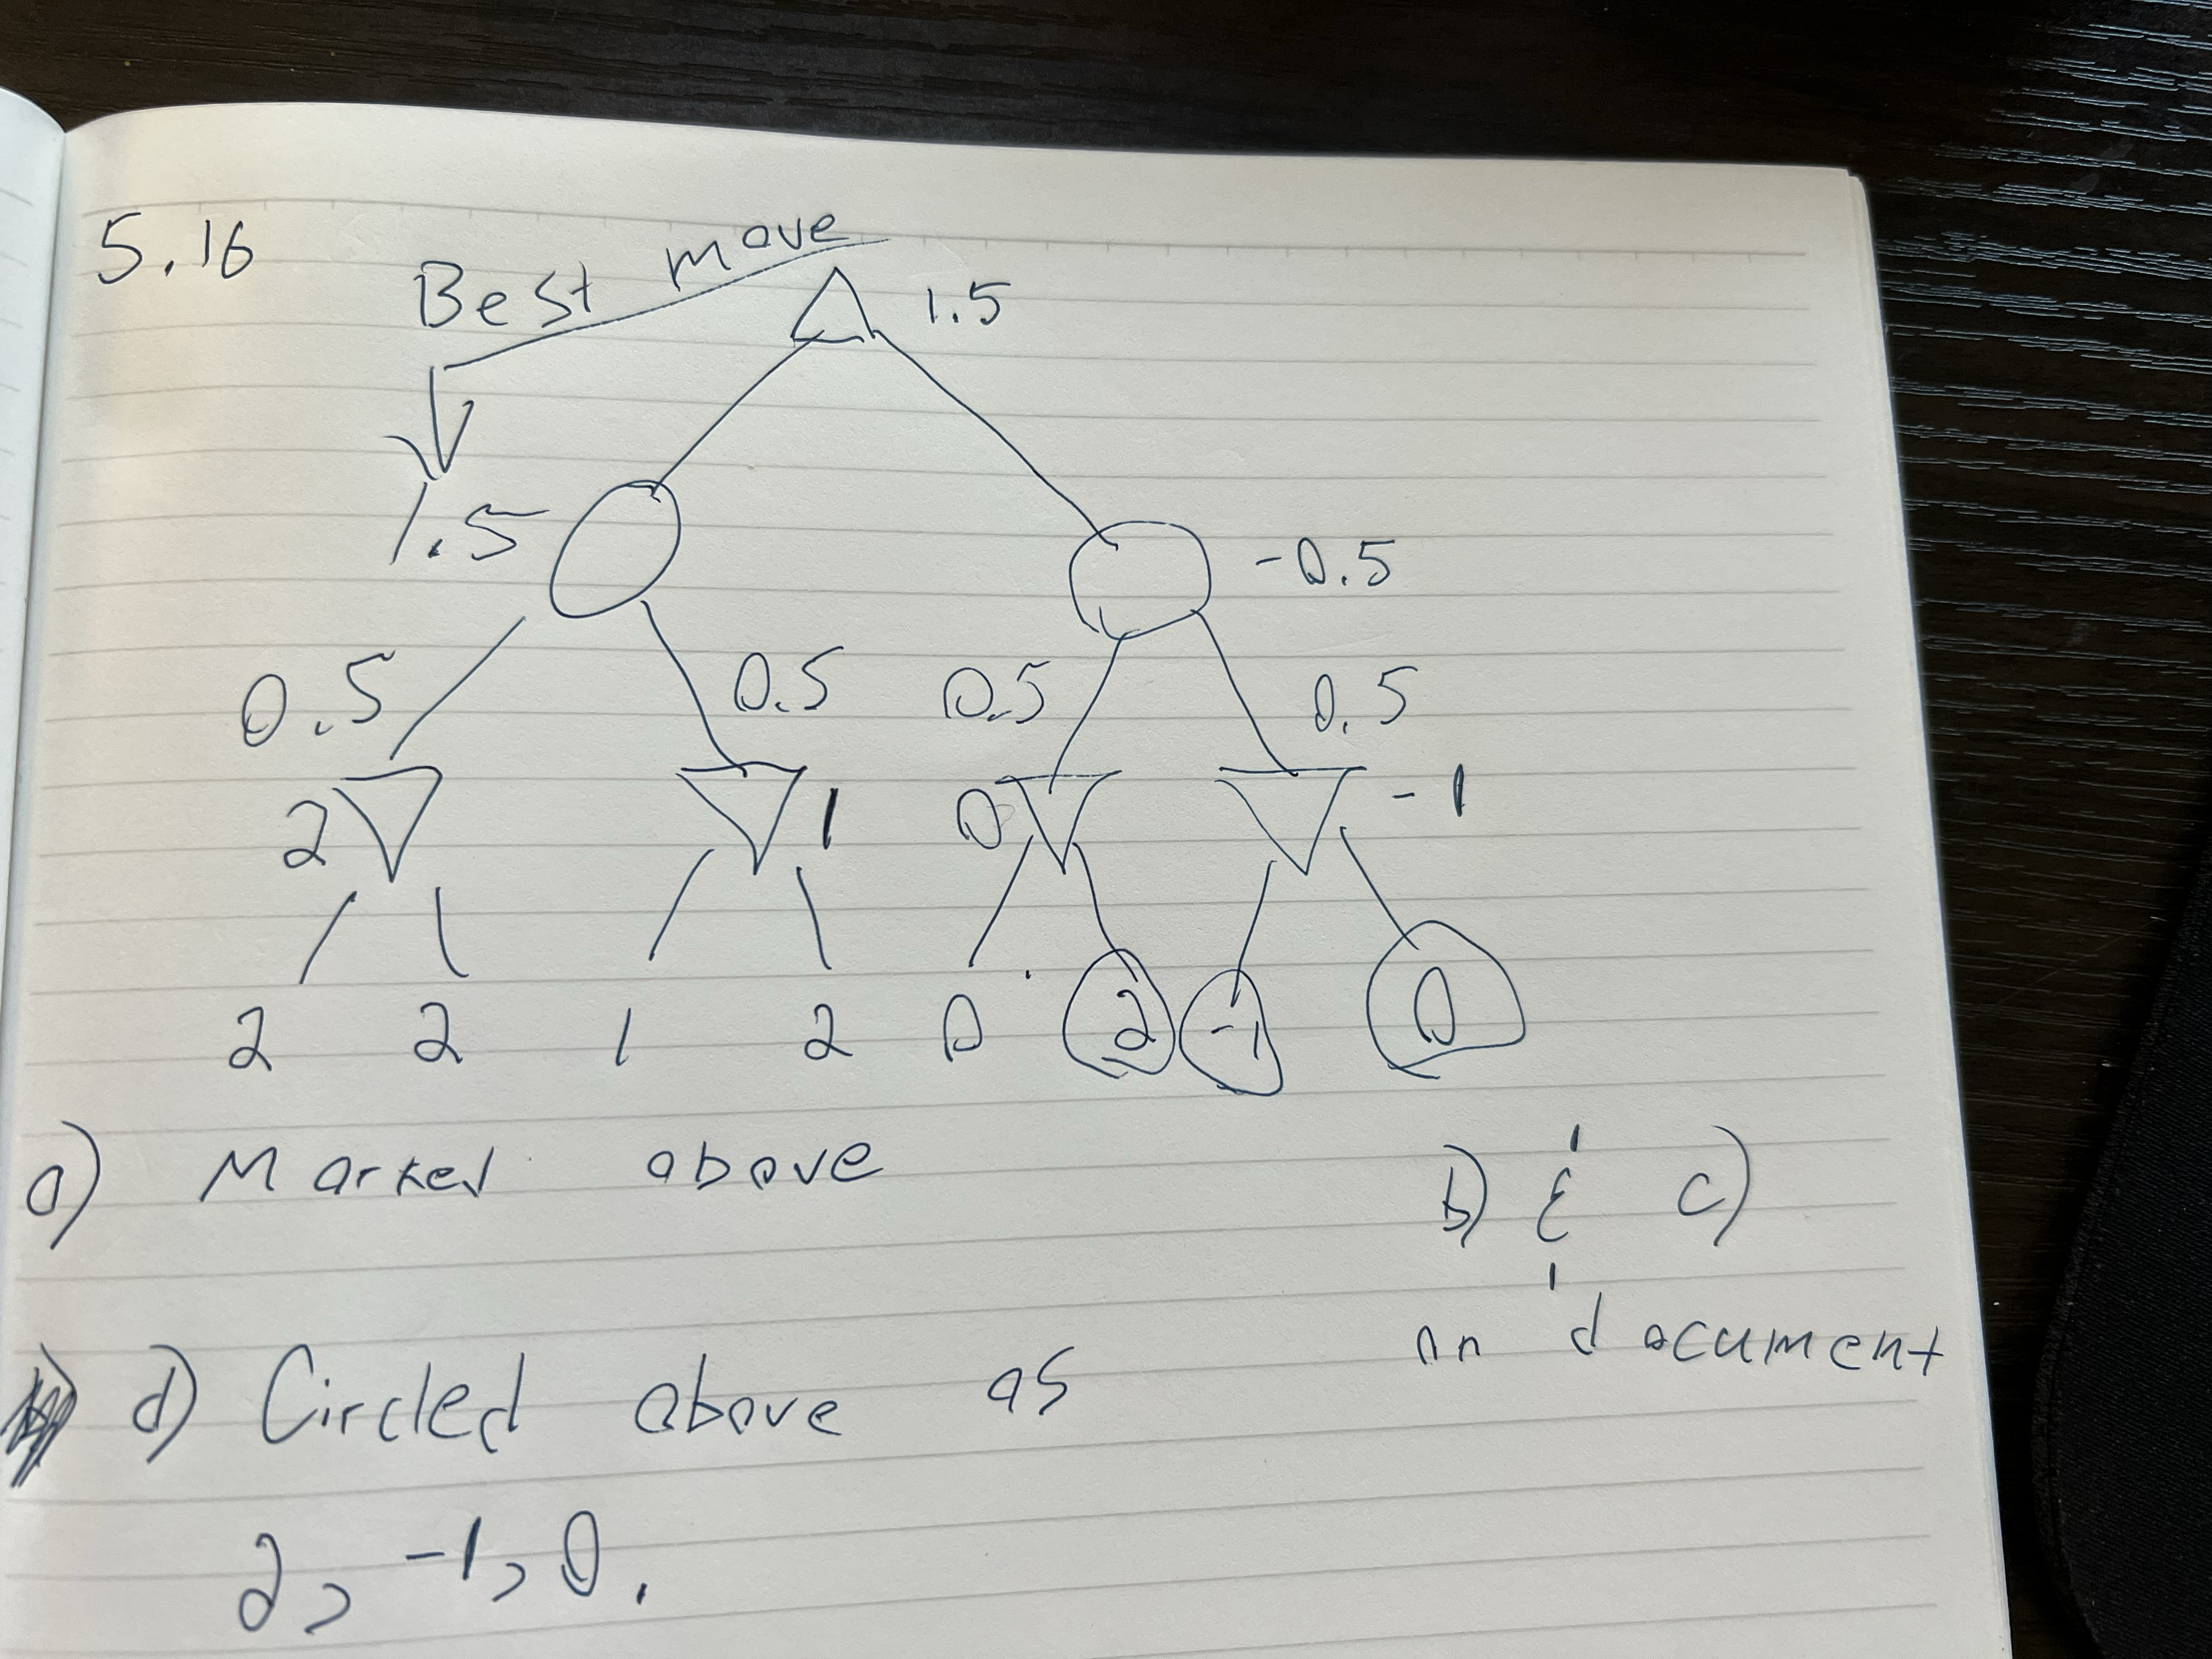
\includegraphics[width=\textwidth]{q516.png} 
 \textbf{b.}  Even if we are to know the first six values of the leaves, we still need to check out the seventh and eighth leaves. There exists a chance that an optimal move will change if nodes seven and eight are very high. This would make the change node valuation much higher than it is, and might make the right side the optimal pathway for the player of the game. If we are given the first seven nodes here, we would not need to visit the eighth node. The chance node value above will not significantly enough to alter the tree. Even if we assume a very high value for node eight, the -1 on node seven will be chosen.
   \hfill \break
   
    \textbf{c.}  We would say the left hand node here after exploring the first two leaves would have a maximum possible value of 2, and a minimum value of 0. The next two leaves will at most be 2, or at least be -2. 
   \hfill \break
   
   \textbf{d.}  I chose the nodes above here on the paper. They were they nodes six, seven, and eight. The reasoning these are chosen is because the zero value on node five, means that the right chance node will always end up being smaller than the left chance node, even if nodes six, seven, and eight were all equal to the max value of two.

\section*{Question 13.8}


\textbf{a.} $\langle$P($toothache$) = 0.20, P($!toothache$) = 0.80  $\rangle$. This is done by summing the columns for each event.
  \hfill \break

\textbf{b.} $\langle$ P($Cavity$) = 0.20, P($!Cavity$) = 0.80 $\rangle$. These are gotten by summing up each of the given rows in the table.\hfill \break
  
\textbf{c.} $\langle $P($Toothache | cavity$) = 0.60, P($!Toothache | cavity$) = 0.40$ \rangle$. \hfill \break

\textbf{d.} P($toothache \vee catch$) = 0.416 . We can use this with the conditional probability formula to obtain what we want.  $ \langle$ P($cavity | toothache \vee catch$) = 0.462, and P($!cavity | toothache \vee catch$) = 0.538  $\rangle$ .
  \hfill \break

\section*{Question 13.13 }
	Determining which test is better can be done by considering a sample size of 10000 people. With a 1\% rate for the virus, 100 people would be infected. In Test A, 95 people would be successfully identified as having the virus, for test B 90 people would be identified as having the virus. However for test A 5 people, and in test B, 10 people would have the virus but never be identified. Additionally, in test A, 1000 people would be test as positive virus cases, but do not have the virus, in test B's case 500 people would be demonstrated to have the virus, but not have it. In total, for Test A, 1005 people were incorrectly identified as what they were, and in Test B, 510 people were incorrectly identified for their conditions. As more people were incorrectly identified in Test A, we can say Test B is generally more indicative of if a patient has a virus or not.
     
\section*{Question 13.15}
Since the test is 99\% accurate, the 1\% inaccuracy in a sample size of 10000 as the doctor mentions would translate to 100 people. This means that 100 people are incorrectly diagnosed with the disease.  There exists a much higher chance that the patient is incorrectly diagnosed, as this is a 1\% chance, versus actually having the disease, which is a 0.01\% chance. 

\section*{Question 14.8}
\textbf{a.} I added the two new variables to the network below.
  \hfill \break
 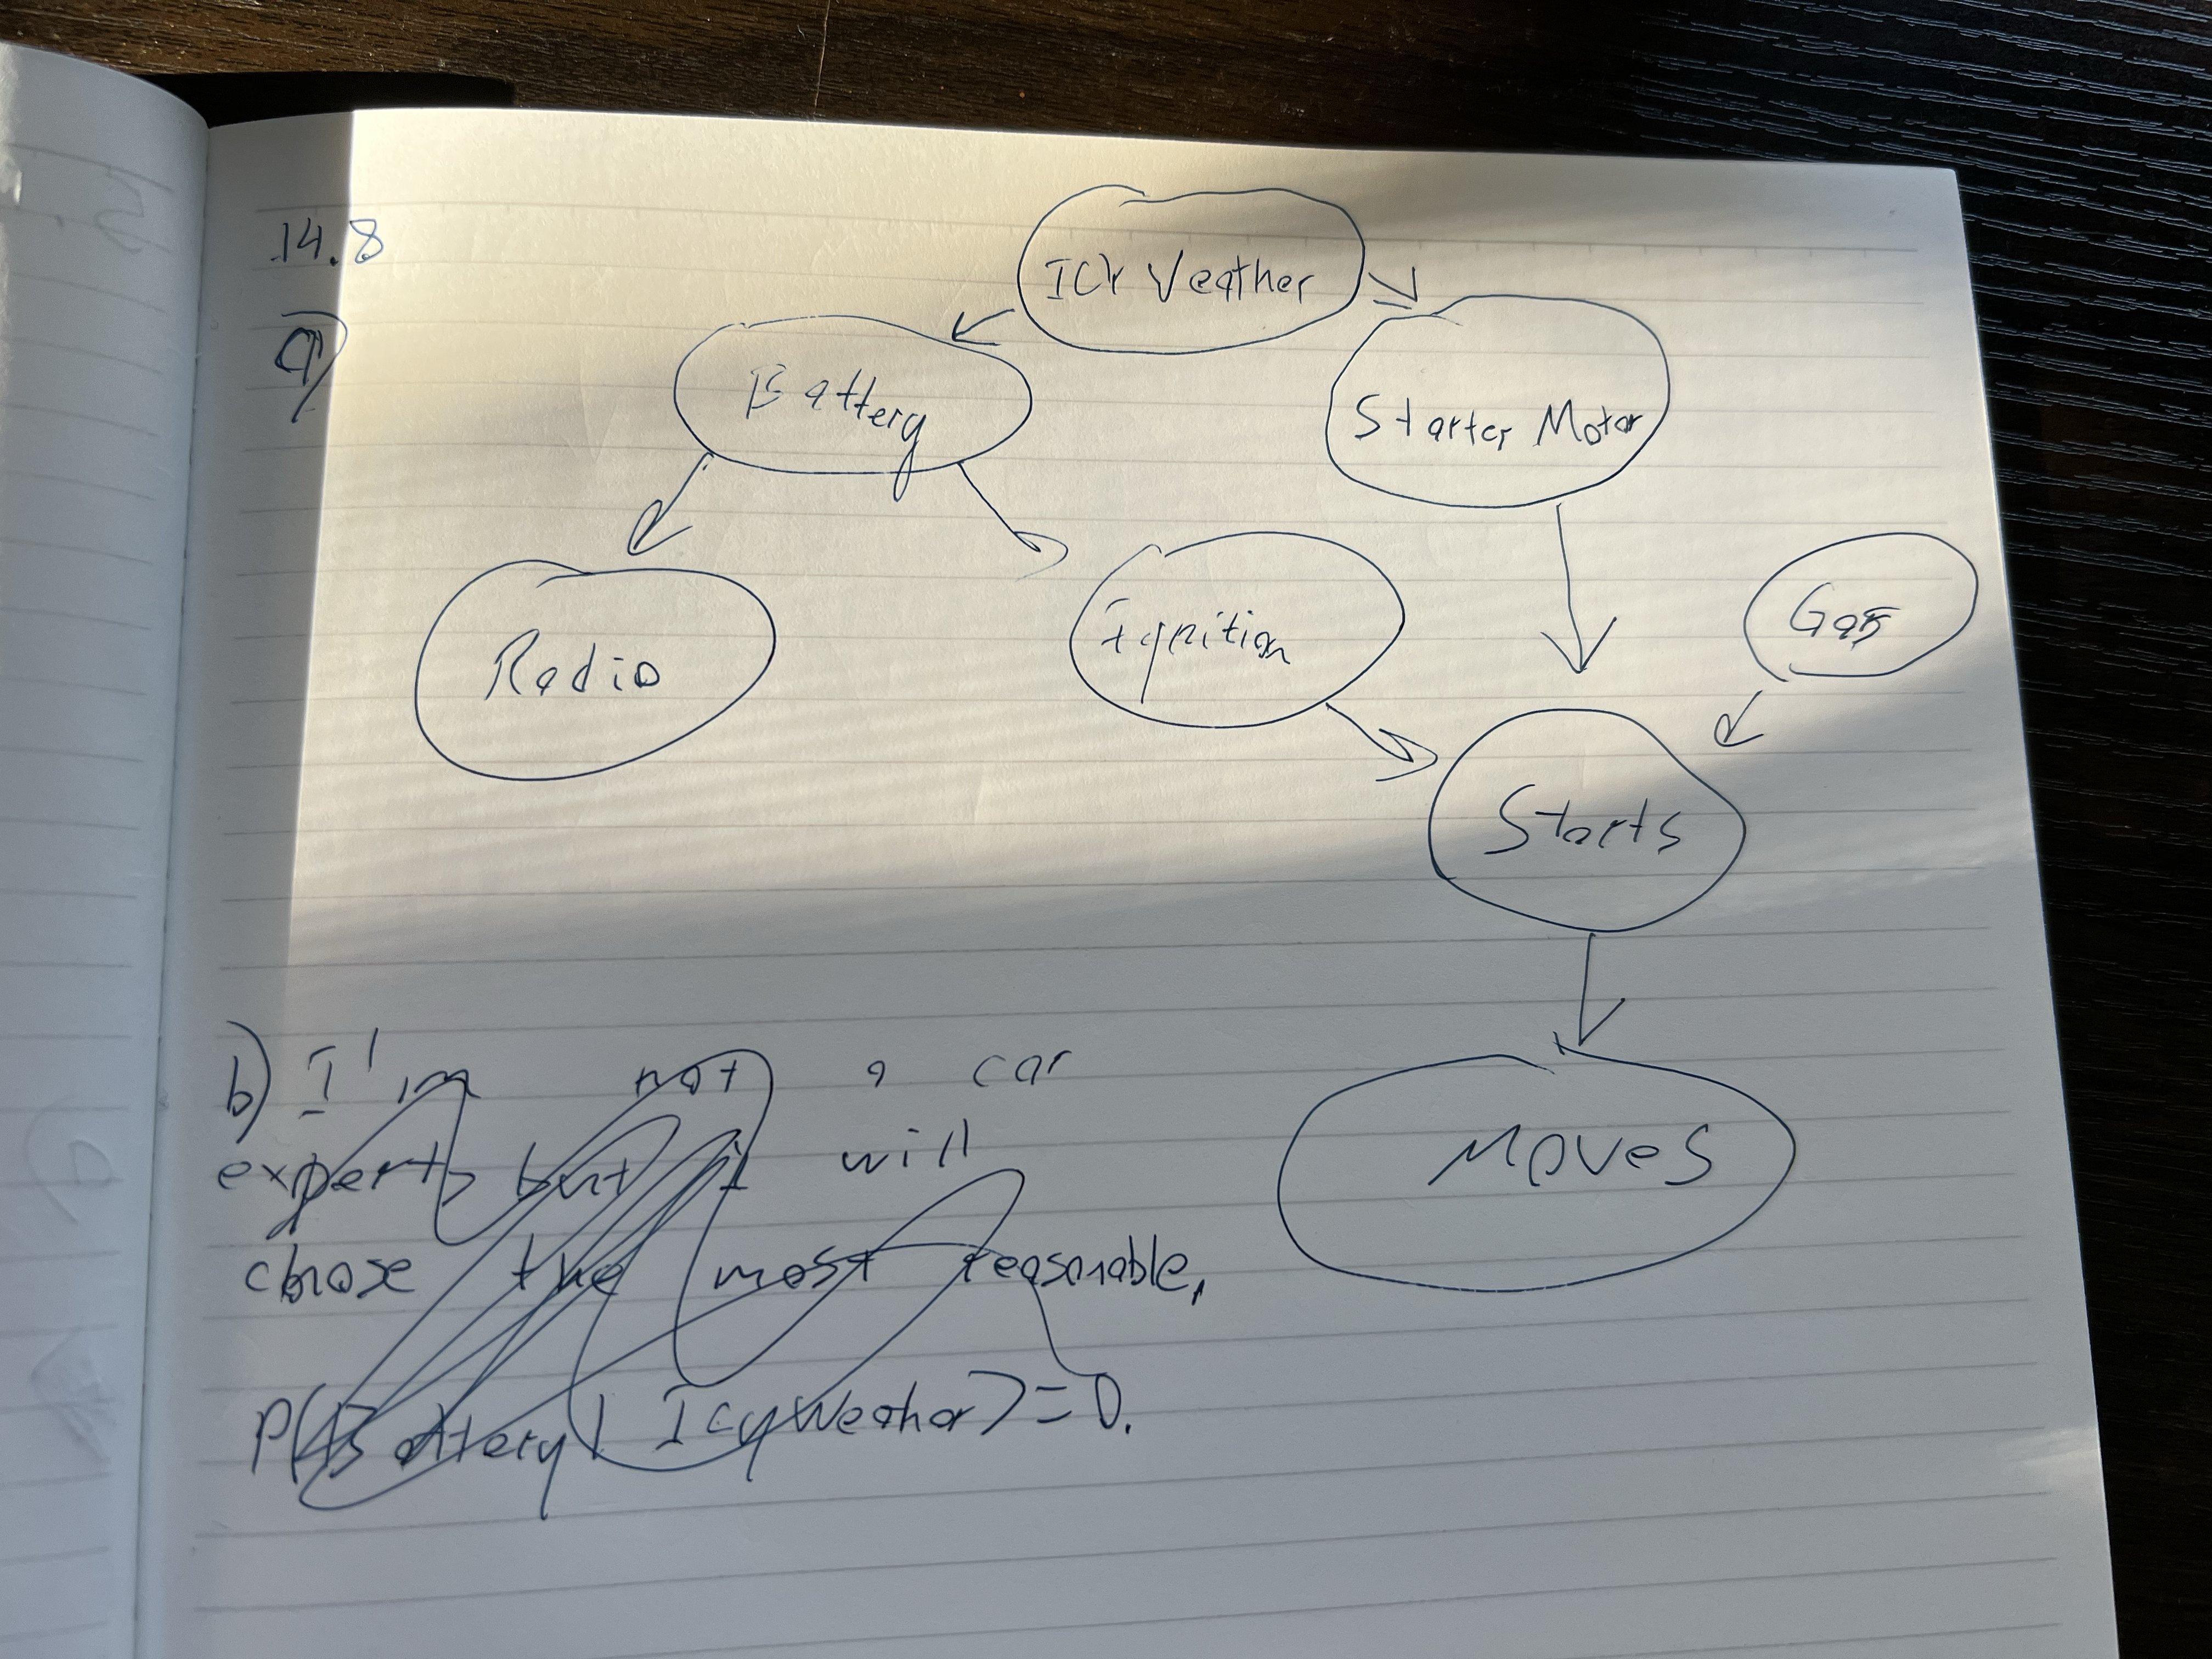
\includegraphics[width=\textwidth]{148.png} 
\hfill \break
 \textbf{b.}  
 ! notates not of an event. I have no car knowledge, but I tried to have estimated reasonable guesses here.
 \begin{itemize}
 \item P($IcyWeather$) = 0.10 (In Canada)
  \item P($Gas$) = 0.94 
  \item P($Radio | Battery$) = 0.98, P($Radio | ! Battery$) = 0.01
  \item P($Ignition | Battery$) = 0.92, P($Ignition | !Battery$) = 0.03,
  \item P($Starts | Ignition, Starter Motor, Gas$) = 0.96, Any other possibility we say the probability of car starting is zero as a car requires each of these things to physically work.
 \item P($Moves | Starts$) = 0.98, P($Moves | !Starts$) = 0.03
 \item P($Starter Motor | IcyWeather$) = 0.93, P($Starter Motor | !IcyWeather$) = 0.98
  \item P($Battery | IcyWeather$) = 0.91,  P($Battery | !IcyWeather$) = 0.98
\end{itemize}

\hfill \break

\textbf{c.} There are 255 different independent numbers amongst the eight variables. $2^8 -1$ = 255.

  \hfill \break
  
\textbf{d.} For each variable with a parent, there are a $2^{parent \#}$ possible events. Using this we can sum up how many table values exist. We have

\begin{equation*} 
2 + 2 + 1 + 2 + 2 + 8 + 1 + 2 = 20.
\end{equation*}

We have 20 independent probability values.

  \hfill \break



\end{document}